\part{Synthesis}
	\chapter{Introduction}
	Now that the relevant product fields are understood to a sufficient degree and the product's needs have been established we can begin to plan out how we will achieve the project's objectives. First we will established the methological approach that will structure the product's development. Then, for each of the core product requirements we will look at a high level design overview of how the requirement will be met, the actual implementation of this design, and testing to evaluate how well this requirement has been satisfied by this implementation.
	
	\chapter{Methological Approach}
	\label{synthesis:methodology}
	The project employed a prototyping methodology for development. First, we must perform an investigation into the system requirements, which was performed in the analysis with a list of specific core requirements being outlined in the conclusion. Following this the first prototype is built, which will resemble an incredibly basic scaled down version of how the final system should ideally look. This prototype is then thoroughly evaluated, with potential changes that would bring the prototype closer to the final system being figured out. Finally, these changes are then implemented and the prototype is evaluated once again. This is repeated until the product has reached its ultimate goals.
	\begin{figure}[h]
		\centering
		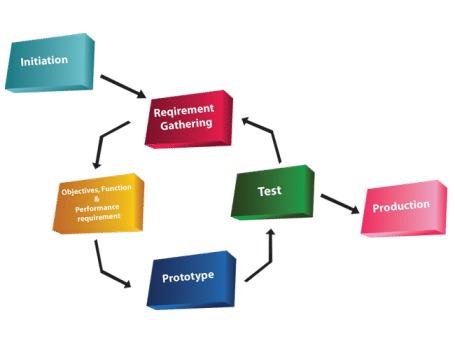
\includegraphics[width=.8\linewidth]{SYNTHESIS/prototypingdiagram.png}
		\caption{Prototyping Methodology}
		\label{fig:prototypingdiagram}
	\end{figure}
	
	This methodology was employed partially due to the hardware nature of the product. Key features of the robot hinged on aspects like movement and observation being possible, so it was important to get a prototype that has this basic functionality up and working and quickly as possible. The prototyping approach allowed a pure focus on getting these functions working, and once they were the robot could be improved iteratively.
	
		\subsection{Initial Prototype}
		As previously stated, this methodology involves an initial prototype that all future prototypes will be an iteration of. The initial prototype of the project will involve the basic, primary construction of the robot. This will first involve the basic chassis assembly followed by attempting to connect relevant components to eachother. Once this is done, we'll hopefully have an incredibly crude robot that won't be capable of anything, but should hopefully serve as a solid foundation for future development toward the project goals.
		
		A similar approach will be followed for processing the map data. It won't be developed simultaneously at first as the robot needs to be capable of storing observational data from the LIDAR before the program can actually do anything, however it will start to be put together once the robot crosses this developmental threshold.
	
	\chapter{Design}
	% QUESTION FOR DAVID --- The design has been written as if the robot is self navigational. is that correct? should i change it?
		\section{Introduction}
		Before implementation of the specific project aims can be implemented, we first need the initial prototype that we can begin iteratively improving. Therefore, it's logical to design the initial robotic prototype first. What follows is an overview of how the initial robot prototype will be designed, followed by a breakdown of each of the individual project aims will be met.
	
		\section{Initial Overview}
		Here will be the design for a high level overview of the project, first establishing the basics of how the robot's structure will be assembled and how the robot's core software will be made.
		
			\subsection{Hardware}
				\subsubsection{Chassis}
				First off will be the basic assembly of the three wheeled omnidirectional chassis. The chassis is comprised of two triangular metal plates, which will be joined together by screwing metal rods into pre drilled holes on each of the platforms. The lower platform is where the motors and mounting points for the omnidirectional wheels are found, so once the plates have been connected the wheels will be pushed onto these mounting points and locked into place. Fig \ref{fig:chassisassembly} shows the assembly document that came with the chassis.
				\begin{figure}[h]
					\centering
					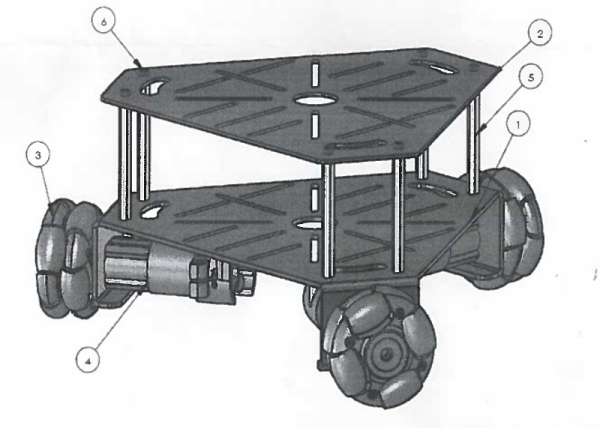
\includegraphics[width=.9\linewidth]{SYNTHESIS/chassisassembly.png}
					\caption{Chassis assembly guide}
					\label{fig:chassisassembly}
				\end{figure}
				
				Now it's time for the microcontroller setup. The microcontroller used in this project is the FRDM-K64F, chosen for its free availability from the University loan office, small form factor and compatibility with the Micro C Operating System which is being employed for the robot's core program. To control the robot we'll also need a motor driver. The dfRobot Quad Motor Driver Shield is being employed for this project, it can be obtained from Amazon for around \pounds{13}. It was chosen for this relatively low cost, the easily available documentation and the fact that it can easily plug into the FRDM-K64F, the microcontroller of choice for this project. This shield will be lined up to the appropriate pins on the K64F and plugged in, in preperation for using the microcontroller to drive the motors. 
				
				The assembly shouldn't be overly complex, no soldering should be needed to connect components so it should be mostly a case of fitting things together.
				
				\subsubsection{Power}
				The hardware components that will need powering are the three motors used to drive the omnidirectional wheels, the microcontroller, and the LIDAR sensor. Table \ref{table:1} has a run down of these hardware components, the voltages, and the milliamp consumption that they have.
				
				\begin{table}[h]
					\centering
					\begin{tabular}{|| l | l | l ||} 
						\hline
						Component & Voltage & Milliamp \\ [0.5ex] 
						\hline
						3x DC Coreless Motor  & 12V & Up to 1400 mA  \\ 
						FRDM-K64F  & 5 to 9V &  50 mA \\
						RPLIDAR  & 5 to 10V & Up to 1050 mA\\
						\hline
					\end{tabular}
					\caption{Components and respective voltages}
					\label{table:1}
				\end{table}
				
				To save on cost and complexity, it would be ideal to only use a single battery for the robot's power source. A single power source will be used for the robot, a battery holder containing 8 1.5V batteries will give us the 12V we need for the motors. Then, a step down voltage regular will be used to lower the voltage required for the other components. A 7v and two 5v currents will be needed to supply power to the microcontroller and the LIDAR respectively.
				
				Generally cheaper alkaline batteries have about 1800 to 2800 mAh (milliamp hours) in them, so an 8 pack of these will give us about half an hour's worth of operation before the robot starts to suffer due to low power. This is a worst case scenario assuming a constant high power draw, but this should be sufficient for the purposes of prototyping and demonstration. 
				
			\subsection{Software}
				\subsubsection{Robot Program}
				The robot's software will be a Micro C OS, implemented using C++ classes and compiled with the mbed SDK platform. Classes will be created based on grouped functionality to allow for greater code readability and efficiency. Once development begins, it would be prudent to create a skeleton OS based on the classes and states outlined by the documentation in \ref{sec:finaldesigndocs}. This will enable confirmation that the software is able to be deployed on the microcontroller, and will serve as a good base for functional implementation.
		
		\section{Designing for Requirements}
		Now that the fundamentals of the hardware's construction and the software's foundations are understood, we can begin to move toward truly fulfilling the project requirements. What follows is an overview of how each of the different project requirements will be met, with appropriate explanations toward the hardware and software employed.
		
			\subsection{Movement}
			The first of the three functional requirements outlined in \ref{requirements:functional} is that 'the robot must be capable of movement'.
				\subsubsection{Hardware}
				The dfRobot Quad Motor shield is being used to help control the motors. Fig \ref{fig:shield} shows an overview of the shield.
				\begin{figure}[h]
					\centering
					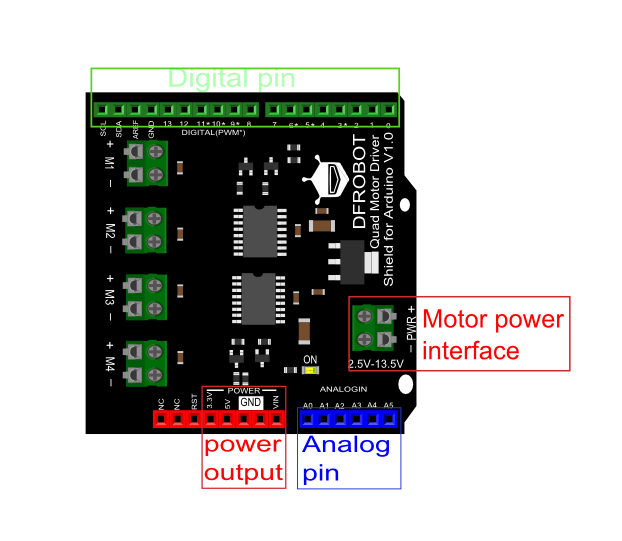
\includegraphics[width=.7\linewidth]{SYNTHESIS/QuadMotorDriverShield.png}
					\caption{Example shield setup}
					\label{fig:shield}
				\end{figure}
			
				The motor power interface is how the shield will actually receive its power from the battery. The power and ground cables from each of the chassis motors will be plugged into the appropriate motor pins that can be seen on the left of the shield figure. Fig \ref{fig:shieldsetup} from the shield's documentation shows an example of this setup with four motors.
				
				\begin{figure}[h]
					\centering
					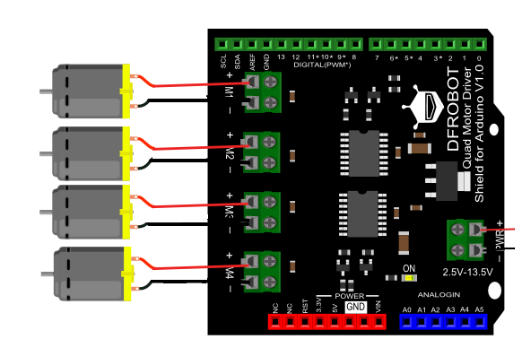
\includegraphics[width=.7\linewidth]{SYNTHESIS/shield_connection.png}
					\caption{Shield connection}
					\label{fig:shieldsetup}
				\end{figure}
				
				Each of the motors power and ground cables will connect to the appropriate pins on the shield. The motors can be manipulated once they receive power in this fashion. The shield is able to affect the electricity being sent to the motors by changing its polarity and by using pulse width modularity. By changing the pin to HIGH or LOW, we can affect the direction that the motor spins in (forward or backwards) and pulse width modulation allows us to affect the speed of the motor.
				
				\subsubsection{Software}
				For each motor on the shield, there are two associated pins. The first of these pins controls the motors direction (forward or backward). The second of the pins controls the motor speed,  achieved using pulse width modulation. To manipulate the motors these pins will need to be declared as variable within the robot's software and assigned different values based on what we are trying to do. The directional pins are either HIGH or LOW, so they will be declared as digital pins that are assigned a binary value. For the speed pins, mbed features a PwmOut interface with a .write() method that can be used to assign a duty cycle value to the variable. This is perfect for what we need. To actually steer the robot, methods in the control class will receive angle and speed values and perform trigonometrical calculations to find out what speed and direction values need to be sent to each of the three motors.
				%talk about pin lineup here and declaration
				% COME BACK TO THIS, TRIGONOMICAL NAVIGATION!
				
			\subsection{Observation}
			The second of the three functional requirements outlined in \ref{requirements:functional} is that 'the robot must be capable of observation'.
				\subsubsection{Hardware}
				Only one range finder is being used to gather the observation data, the RPLIDAR A1M8 LIDAR sensor. The sensor is composed of a platform with a motor system that spins the range scanner as it takes readings, as well as some pins that can be used for communication. Fig \ref{fig:rplidarconfig} illustrates these components.
				
				\begin{figure}[h]
					\centering
					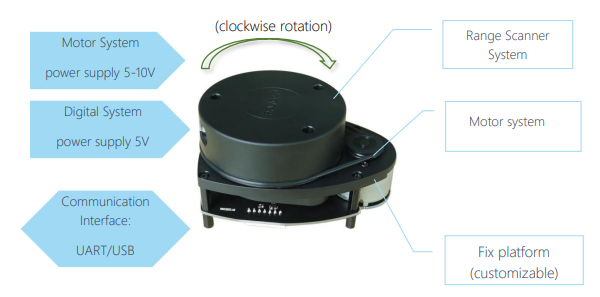
\includegraphics[width=.9\linewidth]{SYNTHESIS/rplidar_configuration.png}
					\caption{LIDAR Underside}
					\label{fig:rplidarconfig}
				\end{figure}
			
				There are seven pins on the underside of the LIDAR sensor, shown in fig \ref{fig:lidarunderside}. These pins need to be connected to the appropriate microcontroller ports if the LIDAR is to work. 
				\begin{figure}[h]
					\centering
					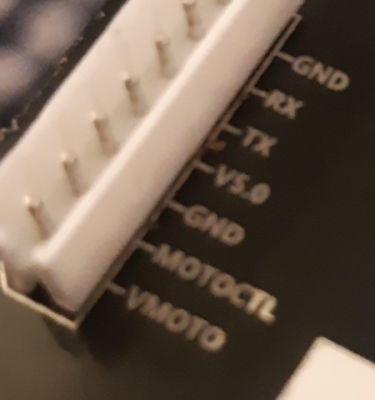
\includegraphics[width=.4\linewidth]{SYNTHESIS/lidarunderside.png}
					\caption{LIDAR Underside}
					\label{fig:lidarunderside}
				\end{figure}
				
				The GND pins are simple ground pins, they will need to be connected to ground pins on the microcontroller. The RX and TX pins (Recieve and Transmit respectively) are serial pins that will be used for communication with the microcontroller. These LIDAR pins will be linked to their opposite counterparts on the microcontroller (LIDAR RX to Microcontroller TX and vice versa). The V5.0 and VMOTO are simple power pins, they will powered via a stepped down 5V current taken from the voltage regulators. This is how the LIDAR sensor will retrieve power. The MOTOCTL pin is the motor control pin that listens for a signal indicating that a connected device is ready to receive data. The signal is either high (ready) or low (not ready). To make use of this pin, a generic GPIO pin from the microcontroller will be configured within the microcontroller's software and set to 1 (high) when the robot needs to begin taking scan data.
				
				\subsubsection{Software}
				\label{sec:observation:software}
				SLAMTEC have a document detailing the LIDAR protocol\citep{rplidarprotocol}. This details the specifics behind how to communicate with the LIDAR. The protocol works by recieving request packets made up of certain bytes. Depending on what the bytes are, the LIDAR interprets the packet as a different command. All request packets contain a one byte start flag and a one byte command field, with optional fields for things like a payload depending on the request being sent. Depending on the command, the sensor will respond in a different way. Fig \ref{fig:examplerequest} shows the documentation's outline of a simple SCAN request which causes the LIDAR to begin outputting observational data.
				\begin{figure}[h]
					\centering
					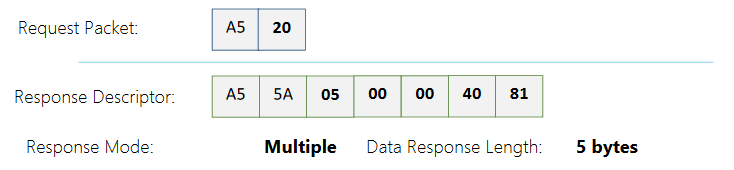
\includegraphics[width=.9\linewidth]{SYNTHESIS/examplerequest.png}
					\caption{Scan Request}
					\label{fig:examplerequest}
				\end{figure}
			
				To begin scanning, a request packet with two bytes of the listed values would need to be sent to the LIDAR. It's advised by the documentation to wait at least 2ms after this before sending any further requests to give the sensor a chance to process the request. Once the sensor has processed the request a response descriptor is sent back. All response descriptors begin with two start flags, and then have five bytes providing information about the coming responses. It provides the size of a single incoming data packet, the send mode of the current request/response session (e.g. single response to the request or multiple responses) and the data type of the incoming response packets.  
				\begin{figure}[h]
					\centering
					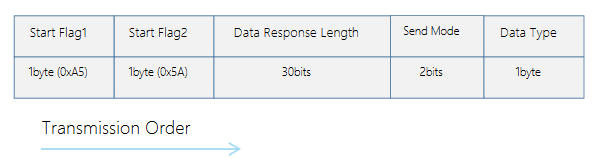
\includegraphics[width=.9\linewidth]{SYNTHESIS/responsedescriptor.png}
					\caption{Response Descriptor}
					\label{fig:responsedescriptor}
				\end{figure}
				
				This could be implemented through the use of data structres in the robot's program. For example, a scan request data structure with two fields (start flag and command) could be initialized and then sent to the LIDAR sensor via the serial connection. Data structures resembling the response descriptors could be populated with information sent back from the sensor as well, allowing for easy processing and manipulation of retrieved data.
				
				This may not be needed however. SLAMTEC provide an SDK for the LIDAR sensor which comes in the form of header files which will automatically implement this functionality. Table \ref{table:sdkbreakdown} has a manifest of the SDK and the functionality that it provides.
				
				\begin{table}[h!]
					\centering
					\begin{tabular}{|| l | l ||} 
						\hline
						File & Purpose \\ [0.5ex] 
						\hline
						rplidar.h  & Parent file for subsequent header files  \\ 
						rplidar\textunderscore driver.h  & Provides RPLidarDriver class for  interfacing with sensor   \\
						rplidar\textunderscore  protocol.h  & Defines structs and constants for the LIDAR protocol  \\
						rplidar\textunderscore  cmd.h & Defines request/answer structs for LIDAR protocol  \\ 
						rptypes.h & Platform independent structs and constants  \\ [1ex] 
						\hline
					\end{tabular}
					\caption{RPLIDAR SDK files}
					\label{table:sdkbreakdown}
				\end{table}
				
				All that would be needed is for the C++ program running on the microcontroller to create an RPLidarDriver variable which would be used to represent the connected LIDAR sensor. Once this is achieved the premade methods that implement the protocol functionality could be ran to achieve control over the LIDAR. Once the LIDAR is retrieving data the class will be able to populate a buffer with readings which can be written to a file once it's full. Readings could also be checked by the robot's main program to see if a distance measurement is particularly low, and if it is the robot could steer away from whatever angle the distance has been measured from to avoid obstacles.
				
			\subsection{Processing Observational Data}
			\label{section:processing:intro}
			The last of the three functional requirements outlined in \ref{requirements:functional} is that 'the observational data must be processed into a map'.
				\subsubsection{Hardware}
				Once the robot is receiving data from the LIDAR sensor, it needs to be transferred to an external program where the CSM software can be ran to generate a map from it. Based on the results of the previously conducted investigation into what would be the most suitable way to store observational data, a Micro SD-Card will be used. The FRDM-K64F has a Micro SD-Card socket attached to it, and the microcontroller will save the observational data to this card so it can be plugged into a machine where it is able to be processed. The University's loans office can provide an 8GB card as well as an adapter allowing it to be plugged into a PC's USB slot, so this approach won't incur any extra cost. The saved data will only be angle and distance measurement pairs, so the card's (relatively) small size won't pose any memory issues. 
				
				\subsubsection{Software}
				First, the microcontroller must save this data to the connected Micro SD-Card. Mbed has a library called SDFileSystem used for interaction with connected SD cards. Using this library, a simple text file will be created on the Micro SD-Card and angle/distance measurements obtained from the LIDAR sensor will be written to it. As the LIDAR scans data it will populate a buffer, and once the buffer has been filled it will be written to the card. After this the buffer will be cleared and begin being populated again. The FRDM-K64F features 256kB of RAM, and a C float is around 4 bytes. If we quite generously assume 156kB will be taken up by task stacks and other program necessities, that still leaves around 100kB of free RAM. In 100000 bytes, we can still store 25000 floats in RAM. Given that each returned scan will probably have two floats (an angle and a distance) we can store at least 12500 readings before the robot needs to pause to write them to file, which should be more than adequate.
				
				Once readings are successfully being obtained and stored to the SD-Card medium, development should focus on turning this data into a map. The first stage will consist of something relatively simple. Converting the measurements into a simple outline or scatterplot graph will allow for some easy visibility on the quality of the readings being retrieved, and will serve as a solid base prototype as developmental focus moves toward making this generated map incorporate multiple scans at different positions. 
				
				To design the GUI, a Python library called Tkinter will be used. It offers all the widgets that will need to be used to make a basic GUI such as frames, buttons and labels and its support of most (if not all) operating systems will allow it to be easily used. To create the regular map to begin with, a Python library called matplotlib will be used. Provided with x and y coordinates, matplotlib can plot these points onto a scatterplot graph. If the angles and distances are converted into appropriate x and y coordinates it should be relatively straight forward to produce a map early on. Once this has been achieved, focus should be turned to implementing CSM for a true SLAM product. The GUI's job at that point is to create an appropriate input for CSM and to use it to generate a map from the readings. CSM takes in readings in the form of either a json or a carmen log. Of the two, json will be used due to its familiarity and much more easily accessible documentation around the internet. To invoke the CSM software itself via the program, Python features a subprocess module which allows for Python programs to spawn simple subprocesses and retrieve information they return. Once the software has processed a map from the readings, it will be output onto the screen so that the user can view it.
		\newpage
		
		\section{Final Design Documentation}
		\label{sec:finaldesigndocs}
			\subsection{Class Diagram}
			Fig \ref{fig:classdiagram} shows the intended classes for the robot's software.
			\begin{itemize}
				\item \textbf{Robot} - The core of the robot's program, this will contain the initial OS setup and the main task which will delegate commands to the Control and Lidar classes.
				\item \textbf{Control} - The Control class will deal with manipulation of the robot's motors. It will contain the relevant variables for each of the motor's direction and speed pins, and given an angle and speed will calculate the necessary values that need to be assigned to these pins to steer the robot in the right direction. 
				\item \textbf{Lidar} - The Lidar class will handle the robot's operations with the sensor. It will store relevant variables for the sensor's operation such as the DTR pin variable allowing it to signal that it is ready to receive data from the sensor, and relevant serial variables to actually retrieve this data from. It will also contain a buffer which it will populate with readings before having them written by its fileWriter class. It will have methods to start and stop the LIDAR's scanning, a method to actually store the readings in the buffer and a method that returns the latest reading for obstacle detection. It will also have some methods that act as wrappers for the SDK's functionality such as getHealth() and getInfo().
				\item \textbf{FileWriter} - The FileWriter class deals with writing the data to the robot's Micro SD-Card. It will have a declaration of the SDFileSystem class provided by the library of the same name, and when supplied with a populated readingsBuffer by the Lidar class it will write the values in the buffer to the SD-Card.
			\end{itemize}
			\begin{figure}[ht]
				\centering
				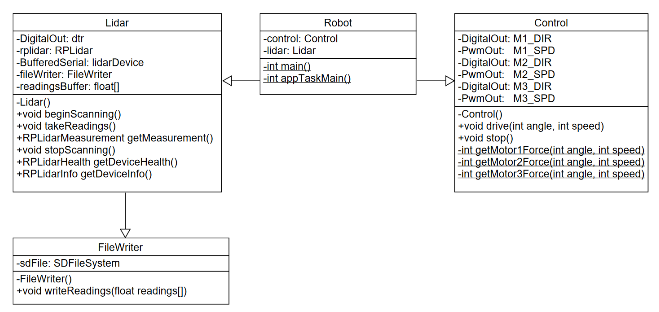
\includegraphics[width=\linewidth]{SYNTHESIS/classdiagram.png}
				\caption{Class Diagram}
				\label{fig:classdiagram}
			\end{figure}
		
		\section{State Machine}
		The finite state machine in \ref{fig:statemachine} represents the different states that the robot can be in.
		\begin{itemize}
			\item \textbf{Initialize} - Setup of variables and tasks once the robot receives power.
			\item \textbf{Scan} - Retrieving observations from the LIDAR and populating buffer.
			\item \textbf{Obstacle Detected} - Recieved measurement has a very low distance.
			\item \textbf{Save Data} - Once the buffer is full it's written to a file.
			\item \textbf{Move} - Moving away from obstacles.
		\end{itemize}
		
		\begin{figure}[ht]
			\centering
			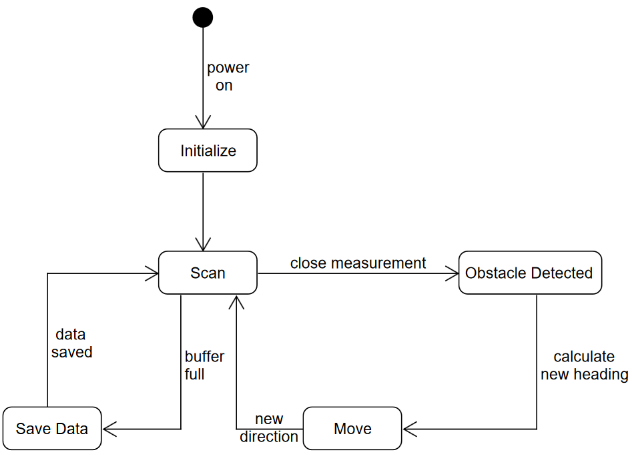
\includegraphics[width=.8\linewidth]{SYNTHESIS/statemachine.png}
			\caption{Finite State Machine}
			\label{fig:statemachine}
		\end{figure}
		
	\chapter{Implementation}
		\section{Introduction}
		This chapter will describe the actual creation of the product. The implementation of relevant software and hardware features for the different product components will be discussed, as well as unforeseen problems that were encountered.
		
		\section{Initial Setup}
		Before work can begin implementing any specific functionality for the robot, some preliminary hardware assembly and software setup had to be carried out.
			
			\subsection{Hardware}
			First of all the physical chassis had to be assembled. The available documentation for the chassis' construction is \ref{fig:chassisassembly} which came in the chassis box. Construction was relatively straight forward and the diagram was of help with a few parts, so it only took around thirty minutes to assemble the structure. Once it was built, the wheels where pushed onto the motors where they clicked on. The Quad Motor Shield was then installed onto the K64F microcontroller without any problems.
				
			\subsection{Software}
			A basic Micro C OS was created and deployed onto the microcontroller. This OS resembled the pseudo code and was composed of skeleton tasks and classes with method stubs.
			
		\section{Implementing Requirements}
			\subsection{Movement}
				\subsubsection{Hardware}
				First the dfRobot Quad Motor shield was fitted onto the K64F microcontroller and placed in the lower level of the robot. Each of the three wheel motors had a ground and a power cable attached to them, these were all fed through the hole in the centre of the lower plate and connected to the appropriate ports on the motor shield. In the interest of keeping the components tidy, the power and ground cables were fastened to the lower plate with zip ties.
				
				Each pair of power and ground ports are labelled with a number on the shield (e.g M1, M2 etc). From hereonn in, the motors will be referred to with these same numbers. Fig \ref{fig:robotwheels} shows the position and names of each of the wheels on the robot.
				% FIG HERE
				
				
				At this point it was time to power the motors by connecting the 12V battery pack to the motor shield. Initially it was planned that this would be achieved from a breadboard, as the breadboard would allow the use of voltage regulators to supply lower voltages to the other components. A problem was encountered here though in the way of space. The microcontroller, motor power cables and battery pack alone already cluttered nearly all of the lower level of the robot. The additional of a breadboard with voltage regulators and additional wiring would be an incredibly difficult fit with wires potentially breaking or coming loose, and there was still the matter later on of connecting the LIDAR properly. This resulted in two decisions being made. The first was that the LIDAR would simply receive power from the microcontroller. The second decision was that the microcontroller would receive its own battery. The K64F features a VIN pin for power that takes between 5V and 9V, so a 6V battery pack was obtained. The power cable was connected to the VIN, and the ground cable shared a ground port with the motor's battery pack. Preliminary tests confirmed that the motors responded to commands sent to them by the robot's software.
				% LINK TO TESTING
				
				\subsubsection{Software}
				\label{req:movement:software}
				Each of the three motors were now connected to two pins on the Quad Motor Shield. One pin affected direction, the other affected the speed. Direction was a simple case of polarity. Depending on the motor, HIGH or LOW dictated whether the motor span forwards or backwards. These pins could be declared as DigitalOut variables, and assigned either a 1 or a 0 depending on what was needed.  The pins that affected speed did so via pulse width modulation, so these could be declared as PwmOut variables and floats could be assigned to them to affect their duty cycle. The motor driver's documentation has a table stating which of the pins on the shield corresponded to which motors, so whichever K64F pin was connected to the relevant shield pin was used for the variables. These variables were declared within the control header and cpp files.
				% state specifically which pin for each motor or is that too granular?
				\begin{lstlisting}
				DigitalOut  M1_DIR(D4);
				PwmOut      M1_SPD(D3);
				
				DigitalOut  M2_DIR(D12);
				PwmOut      M2_SPD(D11);
				
				DigitalOut  M3_DIR(D8);
				PwmOut M3_SPD(D5);
				\end{lstlisting}
				
				Stubs of the methods listed in \ref{fig:classdiagram} were created for the class. Some basic movement methods were made to ensure the robot could actually navigate, making it go forwards and backwards but the ideal implementation involved movement being possible for every heading in a 360 degree radius. Some preliminary problems with calculating force values came up as an issue however. Most force calculations resulted in a raw float values between -1 and 1, but this couldn't be assigned to a speed spin because the pins only supported positive value. Forward and backward motion was dictated by the directional pin. Issues involving other project components ate up time as well, and this aspect of the project was accordingly never fully realised. These problems are explained in \ref{evaluation:processevaluation}.
				
			\subsection{Observation}
			Implementation of the robot's ability to take observations about its environment first involved a hardware configuration. The LIDAR sensor needed to be connected to the microcontroller so that it could draw power from the battery, as well as communicate with the microcontroller allowing it to receive commands and send observational data. Once the hardware connection was established, software on the microcontroller had to be capable of operating the LIDAR sensor and recieving its observations.
				\subsubsection{Hardware}
				As previously discussed, the seven pins on the underside of the LIDAR sensor need to be correctly connected up to the appropriate microcontroller pins if the sensor is to be used.
				
				Table \ref{table:4} gives an overview of which LIDAR pins needed to be connected to which microcontroller pins.
				
				\begin{table}[h!]
					\centering
					\begin{tabular}{|| l | l | l ||} 
						\hline
						LIDAR Pin & K64F Pin & Pin Purpose \\ [0.5ex] 
						\hline
						GND  & GND & Ground  \\ 
						RX  & TX  & Serial Communication \\
						TX  & RX & Serial Communication \\
						V5.0 & 5v & LIDAR Core Power \\ 
						GND & GND & Ground \\ 
						MOTOCTL & D7 & DTR (Data Terminal Ready) \\ 
						VMOTO & 3v3 & LIDAR Motor Power \\ [1ex] 
						\hline
					\end{tabular}
					\caption{LIDAR Microcontroller pin setup}
					\label{table:3}
				\end{table}
			
				Due to the dfRobot Quad Motor shield being plugged into the K64F microcontroller, these LIDAR pins need to be connected to ports on the robot shield that are plugged into the appropriate microcontroller pins. Essentially, we look at what port needs to be used on the underlying microcontroller, then plug it into the motor shield port that is sitting on top of it. The LIDAR pins and shield ports were connected using simple male to female connector wires.
				
				With regards to power, it was previously mentioned in the movement implementation that due to spacial constraints the LIDAR would recieve power from the microcontroller. The microcontroller features two pins that can supply a voltage, a 5V pin and a 3V3 pin. Both pins would ideally recieve 5V, but to save room and ensure a simpler robot the scanner motor was connected to the lower voltage pin. It was decided that the scanner motor should recieve the lower voltage because it only appeared to make the scanner move a bit slower, whereas there was a concern that supplying the actual LIDAR core with a lower voltage might result in problems performing the actual scanning. 
				
				Once this was done, the LIDAR was able to function mechanically.
				
				\subsubsection{Software}
				Following the hardware setup the microcontroller needs to actually communicate with the LIDAR sensor so that it can send commands, as well as receive observational data. This was the responsibiltiy of the lidar.cpp class.
				
				To first of all ensure the LIDAR is ready to communicate, the previously discussed MOTOCTL pin on the LIDAR needs to be recieving a HIGH signal so that it knows the microcontroller is ready to begin recieving data. The K64F features numerous GPIO pins that can be easily configured for usage in situations like this. One such pin (D7) was declared as a basic DigitalOut allowing the microcontroller to manipulate the pin's polarity.
				
				\begin{lstlisting}
				DigitalOut dtr(D7);
				\end{lstlisting}
				
				Simple methods were used for this manipulation. When the sensor needs to output data the pin was set to HIGH...
				\begin{lstlisting}
				void beginScanning() {
					dtr = 1;
				}
				\end{lstlisting}
				
				...or when it had to stop, it was set to LOW.
				\begin{lstlisting}
				void stopScanning() {
					dtr = 0;
				}
				\end{lstlisting}
				
				The microcontroller didn't instantly begin recieving data once this was set up however, as simply connecting the LIDAR and microcontroller serial pins are not enough for communication. In order to interact with the serial channel it needs to be declared in the robot's core program as an appropriate variable. There exists a library for arm MBED microcontroller called BufferedSerial which can be used for this. The original Serial library that it is based on allows for serial communication, with BufferedSerial simply adding a buffer to this. The core functionality remains the same however.
				
				First the pins being used for serial communication need to be declared as a BufferedSerial variable, with BufferedSerial taking the TX and RX pin (in that order) of the microcontroller. It also has an optional baud rate parameter, the LIDAR documentation lists the used baud rate as 115200 so this was supplied just to be safe.
				\begin{lstlisting}
				BufferedSerial lidar_device(D1, D0, 115200);
				\end{lstlisting}
				
				As previously discussed in \ref{sec:observation:software}, SLAMTEC has an SDK that automates most of the LIDAR functionality. The appropriate files were added to the project and made able to be used by the core program with a simple include statement at the top of the lidar.cpp file.
				Following this a base RPLidar variable can be declared from a class the library adds.
				\begin{lstlisting}
				RPLidar lidar;
				\end{lstlisting}
				
				Once this variable has been declared, in the class' main method the DTR is set to 0 to ensure that the LIDAR won't start scanning and outputting data when we don't need it to. The LIDAR variable is then connected to the relevant serial variable (the previously declared BufferedSerial) and the start scan command is issued. Despite receiving the command to start scanning the LIDAR won't begin until the DTR gives it the go ahead, but by configuring this as soon as the program begins it's a lot easier to stop and start the LIDAR data output.
				\begin{lstlisting}
				Lidar::Lidar() {
					dtr = 0;
					rplidar.begin(lidar_device);
					rplidar.startScan();
				}
				\end{lstlisting}
				
				Now that the LIDAR is configured and can begin sending out data, it's time to start actually storing it within the program. First we need appropriate mediums for the storage of LIDAR data. This entails something to store a LIDAR sample that has just arrived so we can manipulate it to take what we need from it, and also a buffer to store all the total readings collect so that they can later be written to disk. 
				
				In order to store a newly recieving reading, the RPLidar SDK implements a basic struct that can be filled in with a .getCurrentPoint() method. This will be used so that recieved readings can be easily manipulated.
				\begin{lstlisting}
				struct RPLidarMeasurement
				{
					float distance;
					float angle;
					uint8_t quality;
					bool  startBit;
				};
				\end{lstlisting}
				
				Now a buffer is needed to store the readings so that they can be written to disk later on. A large number would be preferable so the robot doesn't need frequent stops to save them to the SD-Card. Initially a two dimensional array was used but there was some difficulty in supplying it as a parameter to the fileWriter class, so two large arrays of floats were used.
				\begin{lstlisting}
				float angles[8000];
				float distances[8000];
				\end{lstlisting}
				
				Now that readings can be manipulated and stored, it's time to properly implement the method that stores them to a buffer.
				\begin{lstlisting}
				void takeReadings() {
					struct RPLidarMeasurement measurement;
					for(int i = 0; i < sizeof(angles); i++) {
						lidar.waitPoint();
						measurement = lidar.getCurrentPoint();
						// Get angle
						angles[i] = measurement.angle;
						// Get distance
						distances[i]] = measurement.distance;
					}
				}
				\end{lstlisting}
				The method iterates through both buffers and stores the angle and distance of each reading it receives.		
				
			\subsection{Processing Observational Data}
			Processing the observational data first involves actually finding a way to take it from the robot. It was determined that the best way to implement this would be via the use of a Micro SD-Card. Once this was done, the data itself needed to be turned into some form of map.
			
				\subsubsection{Hardware}
				The only hardware elements that were needed to implement this functionality were the Micro SD-Card socket on the microcontroller, a Micro-SD card and a USB adapter allowing for a computer to access the files on the SD-Card. The socket was already attached to the microcontroller and no adjustments needed to be made to the hardware for the microcontroller to access it.
				
				\subsubsection{Software}
				A FileWriter class was created to handle the functionality of writing the data in the buffer to disk. In order to access the Micro SD-Card the SDFileSystem library was used, and was incorporated into the program by simply including the main SDFileSystem header. To use the library, an SDFileSystem variable first needs to be instantiated. This variable takes five parameters, four relevant microcontroller pins and a name. Table \ref{table:sdfilesystempins} describes each of the four pins the SDFileSystem needs, the name of the corresponding microcontroller pin and what the pin actually is.
	
				\begin{table}[h!]
					\centering
					\begin{tabular}{|| l | l | l ||} 
						\hline
						SDFileSystem Parameter & K64F Pin & Pin Purpose \\ [0.5ex] 
						\hline
						MOSI  & PTE3 & Master Out Slave In \\ 
						MISO  & PTE1  & Master In Slave Out \\
						SCLK  & PTE2 & Serial Clock \\
						CS & PTE4 & Chip Select \\ [1ex] 
						\hline
					\end{tabular}
					\caption{SDFileSystem Setup}
					\label{table:sdfilesystempins}
				\end{table}
			
				The code risks being unclear if regular pin names are always used, so the relevant pins were first defined into more understandable names. The SDFileSystem variable was then declared.
				
				\begin{lstlisting}
				#define MOSI		PTE3
				#define MISO		PTE1
				#define	SCLK		PTE2
				#define	CS			PTE4
				
				SDFileSystem sd(MOSI, MISO, SCLK, CS, "sd");
				\end{lstlisting}
				
				With this variable the file system on the Micro SD-Card is able to be accessed. The previously described scan task is what populates the readingsBuffer with data that is needed, so a method is required to iterate through the buffer and write the observational data to the Micro SD-Card.
				
				\begin{lstlisting}
				void writeReadings(float angles[], float distances[]) {
					// Create the readings file on the Micro SD-Card
					FILE *fp = fopen("/sd/readings.txt", "w");
					
					// Error checking
					if (fp == NULL) {
						pc.printf("Unable to access/create file \n");
					}
					
					// Iterate through the readingsBuffer and write the angle/distance pairs
					for(int i = 0; i < angles.length; i++) {
						fprintf(fp, "%f %f", angles[i], distances[i]);
					}
					
					// Close file
					fclose(fp);
				}
				
				\end{lstlisting}
				First the fopen method is called with a designated file, and the "w" parameter (meaning write) ensures that the file will be created if it doesn't already exist. Then a basic error check follows to make sure that the file is accessible, followed by an iteration through the readingsBuffer. As was previously mentioned, the buffer is populated by pairs of angle and distance measurements, so for each entry in the array the angle and distance is written to the file. These pairs were written as two values seperated by a comma, with each value being seperated by a space. This was done to make it easier to read from a program point of view. The plan was that the file can be split by spaces to get pairs, and then each pair can be split by a comma to get the individual values. Finally, the file is closed.
				
				As mentioned in \ref{section:processing:intro}, a GUI would be used for the processing of map data. Tkinter is a simple Python package that is capable of quickly creating incredibly basic GUIs. All that was needed was a panel with some buttons that called methods to turn our readings file into a map.
				% get picture of a gui with plain buttons?
				
				The first thing to do was begin generating a plain map. Once a simple map could be made from angle and distance measurements obtained from the robot, this process could be elaborated upon to move toward something more thorough generated by CSM. For this, matplotlib was used. matplotlib would allow the generation of a scattermap and, when supplied with x and y values, would plot appropriate points at these coordinates onto the map. The first task was to convert angles and distances into usable x and y coordinates.
				
				Initially dummy data was used to verify that the process worked. First, data from a .txt file had to actually be read into the program. A button was attached to a simple method that did this.
				\begin{lstlisting}
					# Retrieve distance-angle pairs from a text file
					def readData(self):
						try:
							with open("coordinates.txt") as textFile:
								lines = [line.split() for line in textFile]
								# Values are read in as strings, so we convert them to ints
								for i in lines:
									i[0] = int(i[0])
									i[1] = int(i[1])
									return lines
						
					except IOError:
						print("Error reading file!") 
				\end{lstlisting}
				Angle and distance pair values are read in from a text file. These values are separated by whitespace, so the method iterates through each line in the file and splits each line into two tokens which are kept in an array. These tokens are read in as strings so they are cast to ints.
				
				Once this data was being gathered from a text file it needed to be turned into a plottable x and y coordinate. This was achieved with some trigonometry.
				\begin{lstlisting}
					def getCoords(self, measurement):
						x = measurement[1] * math.cos(math.radians(measurement[0]))
						y = measurement[1] * math.sin(math.radians(measurement[0]))
						return x, y
				\end{lstlisting}
				Each angle and distance pair is turned into its corresponding value on an x and y axis. Now that it was possible to read in data and turn it into a plottable point, it was time to combine this into an actual map.
				
				\begin{lstlisting}
					# Draw map on plot
					def showMap(self):
						measurements = self.readData()
						coords = []
						x = []
						y = []
						
						# Turn distance-angle pairs into usable coordinates
						for measurement in measurements:
							x.append(self.getXCoord(measurement))
							y.append(self.getYCoord(measurement))
						
						plt.plot(x, y)
						plt.show()
				\end{lstlisting}
				This method was attached to a button. It uses the previously described readData() method to retrieve values from a file, turns each of the retrieved measurements into a plottable coordinate, appends it to an array and finally this array is plotted by the matplotlib scatterplot.
				%picture of the test map here
				
				This was as far as this component got in development unfortunately. Issues with other features cost time, and problems were encountered with getting CSM to work. These problems are explained in \ref{evaluation:processevaluation}.
				
	
	\chapter{Testing}
	%Build toward it
		%Does movement work?
		%Does it scan?
			%Compare observation prints to the terminal ones
		%Does it store the scan? How quick?
			%Compare observation prints to the SD card ones
			%measure-mbed for write speed
	
	% QUESTION FOR DAVID --- Code and screenshots for testing programs?
	This chapter will discuss the testing performed on the system. The purpose of the testing is to determine how well, if at all, elements of the implemented work satisfy the requirements outlined in \ref{requirements}. Each test will have its process and purpose described, and based on the results there will be a discussion of how it affected development. These results will also be used for the product's evaluation.
	
	Because the project employs both software which is easy to view and understand, and hardware which in some cases only the results of inputs could be seen rather than how the inputs were actually processed, a mixture of white and black box testing was employed.
	
	In keeping with the developmental methodology outlined in \ref{synthesis:methodology}, tests were carried out at key functional milestones to ensure that what was implemented was robust and appropriate enough to be iterated on by the next prototype. When appropriate, it will be explained what stage of development the project was at during the test.
	%Purpose of testing, what will happen here
	%Nature of testing. Black/white box?
	%Explain the importance of testing in relevance to the chosen methodology
	
	%Iterate the tests at each design stage?
			
		\section{Testing the Movement}
		One of the functional requirements of the project outlined in \ref{requirements:functional} is that robot must be able to move. One of the first aspects to the construction of the robot was implementing its ability to move. At this point in the project it wasn't a fully connected system, so movement ability was being tested in complete isolation. There was no destination in mind, the goal here was to see whether or not the fundamentals behind the microcontroller driving the robot via commands to the motors had been successfully established. 
		
		At this point in the project the robot's movement wasn't sophisticated, and four methods existed to drive the robot in basic directions (forward, backward, left and right). This still needed to be tested however, as any further implementation would be a failure if the fundamentals weren't understood. A test environment had to be created to allow an ability to view what direction the robot was told to go in whenever it moved. A small task within a basic Micro C OS environment was created for this. A random number was picked from zero through to three, with each of the four numbers corresponding to one of the four different movement methods that drove the robot in one of the four aforementioned directions. Once the number had been picked, a simple if statement called whichever number was tied to which method. Which number corresponds to which direction can be seen in table \ref{table:movementtestkey}.
		
		\begin{table}[h!]
			\centering
			\begin{tabular}{|| l | l ||} 
				\hline
				Number & Direction \\ [0.5ex] 
				\hline
				0 & Forward \\ 
				1 & Right \\
				2 & Backward \\
				3 & Left \\ [1ex] 
				\hline
			\end{tabular}
			\label{table:movementtestkey}		
		\end{table}
	
		To verify whether or not the robot is correctly moving based on the randomly generated number, it is plugged into a terminal during the test and a terminal is used to print the randomly generated numbers as they are received over a serial connection. The testing task itself will have print statements to allow the randomly generated number to be seen by the tester.
		
		\begin{lstlisting}
			static void appTaskRobot(void *pdata) {
				while (true) {
					// Random number between 0 and 3
					int direction = rand() % 4;
					
					if(direction == 0) {
						pc.printf("Forward");
						goForward();
					}
					if(direction == 1) {
						pc.printf("Right");
						goRight();
					}
					if(direction == 2) {
						pc.printf("Back");
						goBackward();
					}
					if(direction == 3) {
						pc.printf("Left");
						goLeft();
					}
					OSTimeDlyHMSM(0,0,3,0);
				}
			}
		\end{lstlisting}
		The testing will allow a verification of whether or not the base movement functionality has been implemented properly. If the robot moves in the direction that the program tells it to every time then aspects such as wheel direction toggling, wheel speed and which robot motor pertains to which variable within the robot's code have been understood and implemented properly. If not, the understanding of how the robot's movement works is flawed and will be re-evaluation. This test would be performed for twenty different values, and for each values the printed direction and direction the robot travelled in will be observed.
		
			\subsection{Test One}
			Table \ref{table:movementtestbasic} has the first test's results in depth. Each of the appropriate directions printed to the terminal matched the direction that the robot travelled in. This means that the fundamentals behind how to manipulate the motors to achieve movement has been understood, and that the way in which this is done has been successfully implemented into a form usable by the robot's microcontroller. This only accounts for basic movement however, nothing can be surmised about more elaborate functionality involving true omnidirectional movement. As well, the test does not allow any insight into how well the wheels function once the chassis has more components and wiring in it. This test should be conducted again once the robot has more elements to it to ensure the motor's operations aren't impeded by wires and such.
		
			\subsection{Second Test}
			As previously mentioned and stated in the non-funtional requirements, one of the elements of the robot's build quality is ensuring that the motors operations aren't impeded by other components getting in the way. Once more components were a part of the robot such as batteries and the LIDAR sensor, another test was conducted using the same environment as the first movement test. Attention however was focused on the robot's operation itself, looking to see if it was impeded by loose wires or other elements, but it never was. This test then succeeded, and verifies one element of the robot's build quality.
			
			% QUESTION FOR DAVID ----- Is it worth even talking about a test that wasn't ran?
			\subsection{Third Test}
			The first movement test established the robot's basic movement capability, but ideally the robot would move in an omnidirectional manner. The Control class in the robot's program should feature a method capable of using an angle and speed value to calculate the appropriate force needed for each wheel to move it in that direction at the specified speed. The test environment for this will be very similar to the basic movement test, only rather than generating a single random number between zero and three there will be two randomly generated numbers. The first will be between zero and 360, and the second will be a float between 0 and 1. These randomly generated numbers will then be supplied as parameters to the drive method, as well as being printed to a terminal over a serial connection for observation by the tester. Some slight inaccuracy should be tolerated here, as long as the robot moves within five to ten degrees of the supplied angle at an observably correct speed the test will be considered a success.
		
			Unfortunately this method was never properly implemented, and as such it cannot be tested. This test then is a fail. This means the robot is not capable of omnidirectional movement, which could impede its ability to map an environment which is one of the core functional requirements.
		
		%First test that each of the motors works using vague directions.
			%These will be verified from my personal observations.
			%Test forwards, backwards, left, right, and then do a spinny.
			
			%while true
			%int direction = math.rand(0,4)
			%if direction = 0 go forward
			%if direction = 1 go backward, etc
			
		\section{Testing the LIDAR's Implementation}
		One of the project's functional requirements outlined in \ref{requirements:functional} is that the robot must be capable of observation. The project employed the RPLIDAR A1M8 sensor for observation. Initial testing of the sensor didn't concern accuracy, but rather ensuring basic control of the LIDAR could be achieved via the use of the microcontroller. The environment for this test took the form of a simple Micro C OS task running on the microcontroller, shown below. The microcontroller would retrieve data from the LIDAR sensor and output it to a terminal. Whether or not the distances being produced by the LIDAR sensor were of a certain metric accuracy was incredibly difficult to ascertain, but by moving things around the LIDAR sensor at different angles it was possible to observe whether or not distance measurements were increasing or decreasing at corresponding angles.
		
			\subsection{Test Results}
			The first test was more of a proof of process with regards to LIDAR manipulation. Once the microcontroller task began, data was successfully being printed to the terminal for different angles. The frequency of the printing was significantly lower than the LIDAR's sample rate of 4000 - 8000hz, so a complete spectrum from zero to 360 degrees was not always viewable. Objects were placed around the LIDAR and moved closer to it. It was observed from that that different distance values began decreasing. When the objects were moved away, these values increased again. 
			% we can get a test table for this maybe, move stuff away and closer at different angles
			
		%To get the LIDAR SDK working, a serial terminal was used.
			%Connect LIDAR to microcontroller and print
			%Then the OS started the LIDAR and began printing the values to the terminal.
			
			%Do the same for when the LIDAR is plugged into the motor shield on top of the microcontroller? - naw, have this by default
			
			%Show the test code
			%Say your observations
				%Moved things closer, distances got lower. Moved things away, distances got higher.
			
		\section{Testing the File Writing}
		\begin{lstlisting}
			dtr = 0;
			rplidar.begin(lidar_device);
			rplidar.startScan();
			struct RPLidarMeasurement measurement;
		
			for(int i = 0; i < 10; i++) {
				rplidar.waitPoint();
				measurement = rplidar.getCurrentPoint();
				pc.printf("Distance: %f Angle:%f\n", measurement.angle, measurement.distance);
			}
		
		\end{lstlisting}
		%LIDAR was ran and told to print the first 10 values that it got.
		%Values were then saved to the SD card.
		%USB adapter for the Micro-SD Card was plugged in, values were observed and compared.
			%Were they different? Did they save? What format did they save in?
			
		\section{Testing the GUI}
		%Firstly, does the GUI run?
		%Second, can it read files? Read some test files like the binary coords.
			%Make a .txt file, click a button that reads it and prints it. Do this for 10 random strings.
			%or give it some random coords and see if it maps them mathematically correctly
				%e.g. give an angle and distance, work out what the x and y should be, see if it plots
				%or make random shapes like squares
		%Then, can it read the saved data from the robot?
			%Test this 10 times as well
			
		\section{Testing CSM}
		%Get it working with a test log (DDDDDDDDDDDDD:)
		%Get it working with a test log called from the GUI (DDDDDDDDDDDDDDDD:)
		%Get it working with a real log (DDDDDDDDD:)
		%Get it working with a real log called from the GUI (DDDDDDDDDDDD:)
			
		\section{Testing the System}
		%All of the above.
			%Generates a random number, moves in that direction.
			%Scans and prints data.
			%Saves the data to a Micro SD-Card.
			%Plug that into the PC, see what the GUI says.
			%10 times, change the environment each time.
				
	\chapter{Blockers}
	Any minor issues encountered during development have been touched on in the implementation. Larger problems were encountered however that caused a more significant hindrance to the product's development. Some of these issues even involved the whole developmental approach having to be reconsidered. This chapter aims to explore these issues in depth by detailing what happened and how, if at all, these issues were overcome.
		
		\section{LIDAR Communication}
		A problem encountered near the start of the project was getting the SDK to work with the LIDAR sensor. The SDK's documentation states that the rplidar.h file simply needs to be included to gain LIDAR functionality, but when this was done the program gave file dependency errors during compile attempts. The most prominent error was an import problem where files within the SDK were unable to import the file sys/ioctl.h. Looking into this, ioctl.h appeared to be a linux kernel header file. The first attempt to fix this was simply making sure these kernel files were working properly, so APT was used to install or update the linux kernel headers. Other packages such as build-essentials were also installed, but none of these things fixed the problem. One other potential problem was that maybe there was a program somewhere relying on 32bit libraries which the 64bit Ubuntu OS didn't have, so APT was used to install the i386 architecture as well as some relevant packages to allow for better 32bit support. This didn't fix anything either. In a last ditch effort some of the kernal header files were actually copied into the LIDAR SDK, but this just resulted in other dependency problems coming up.
		
		Rather than continuing to spend time attempting to get the SDK working, it was decided to simply use the actual protocol that the SDK implemented. The protocol works by recieving request packets made up of certain bytes. Depending on what the bytes are, the LIDAR interprets the packet as a different command. These packets were created in the robot's program as arrays of bytes, and the Serial puts() command was used to send them to the LIDAR. getc() was then used within a task's main loop to retrieve the outputted data and it was printed to a terminal window. Relevant code snippets can be seen below.
		\begin{lstlisting}
		Serial pc(USBTX, USBRX);
		Serial device(D1, D0, 115200);
		
		char startRequest[] = {0xA5, 0x20};
		device.puts(startRequest);
		
		while (true) {
			pc.printf(device.getc()); 
		}
		\end{lstlisting}
		This had mixed results. Bytes were being recieved to the LIDAR but they were incredibly inconsistent. There wasn't a steady stream or a regular pattern to what was being returned. As well, bytes would stop coming through if the program was recompiled and reflashed or if the board itself was reset with the reset button. In addition to that the other commands listed in the protocol were even less effective. A stop request can be sent to the LIDAR so that it stops outputting data, but when this was sent any subsequent start requests wouldn't work and the LIDAR would stay dormant. To get the LIDAR working again the program itself had to be reset. The protocol documentation did state that a small period of time should be allowed to elapse between two commands being sent to ensure the LIDAR could process them, but even 3 to 4 seconds worth of a delay didn't fix anything here. Some requests had even more confusing results. The get health request is something that the documentation says returned 3 bytes, but when an appropriate request variable was made and sent to the device over the serial connection it returned only two bytes. Incidentally even if the command did work part of the response is an integer that represents the error code, but nowhere in the documentation could an actual table explaining what error each code corresponded to be found. 
		
		After consultation with the project mentor and some further studying of the Serial class, the potential solution of ensuring that data was retrieved via an interrupt rather than a constant loop presented itself. Having getc() constantly called whenever the while loop ran might have been causing problems, but with an interrupt handler it would only trigger when there was actually something there. Mbed's own documentation describes the RawSerial as a more suitable alternative to Serial for this approach so the device variable was changed to be of a RawSerial type. The code changes can be seen below.
		
		\begin{lstlisting}
		RawSerial device(D1, D0, 115200);
		
		device.attach(&rxInterrupt, Serial::RxIrq);
		
		void Rx_interrupt() {
			pc.printf(device.getc());
		}
		\end{lstlisting}
		This meant that the code to retrieve information from the device only ran when a character went into the RX buffer and was actually ready to be recieved. The strange behaviour with the stop request and some of the other requests was still present, but this resulted in LIDAR data being continuously and consistently printed to the console. This meant that at the very least there was data that could be worked with for now. These numbers were written in a binary representation to the Micro-SD card so they could be processed by the GUI, but there were problems there as well.
		
		This binary data would have to be turned into actual angle and distance numbers however. Fig \ref{fig:protocolbreakdown} is from the LIDAR protocol documentation, giving a breakdown of what byte in a returned scan packet corresponds to what information.
		
		\begin{figure}[ht]
			\centering
			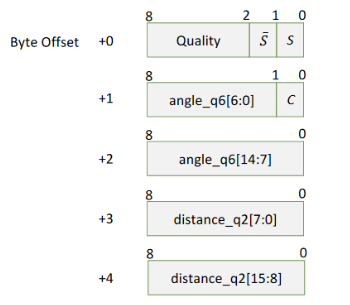
\includegraphics[width=.6\linewidth]{SYNTHESIS/protocolbreakdown.png}
			\caption{Protocol Breakdown}
			\label{fig:protocolbreakdown}
		\end{figure}
	
		So, for example, the first 6 bits of the first returned byte is used to store the scan's quality value. The idea behind the initial map processing software was to start at the beginning of the file containing binary scan data, then iterate through it by taking chunks of bits and storing them in variables.
		
		\begin{lstlisting}
		# Read in the bits according to the LIDAR response structure
		quality = f.read(6)
		inverseStart = f.read(1)
		start = f.read(1)
		angle_first = f.read(7)
		checkbit = f.read(1)
		angle_second = f.read(8)
		distance = f.read(16)
		\end{lstlisting}
		One small additional tweak that needed to be made was joining the first and second angle chunks together to form the full value.
		
		\begin{lstlisting}
		# Append the angle_q6 bits
		angle = (b"".join([angle_first, angle_second]))
		\end{lstlisting}
		
		The protocol documentation states that these aren't the true values however. The actual angle value is the binary value divided by 64 degrees, and the actual distance value is the binary value divided by 4 millimeters.
		
		\begin{lstlisting}
		# Turn binary into decimal
		# 'Actual heading = angle_q6/64.0 Degree'
		angle = (int(angle, 2) / 64.0)
		# 'Actual Distance = distance_q2/4.0 mm'
		distance = (int(distance, 2) / 4.0)/100
		\end{lstlisting}
		These points were then turned into mappable X and Y values. Despite all of this, none of this worked as intended. The produced maps made no logical sense, fig \ref{fig:failedmap} shows a map produced via this method from scans obtained from the inside of a rectangular box.
		\begin{figure}[ht]
			\centering
			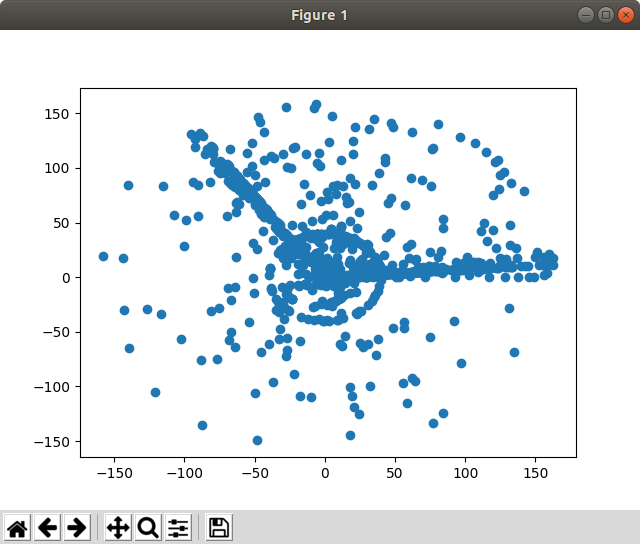
\includegraphics[width=.6\linewidth]{SYNTHESIS/failedmap.png}
			\caption{Resulting map of a box}
			\label{fig:failedmap}
		\end{figure}
	
		The generated values were printed, and it was observed that every now and then angles would be impossible values above 360. After all of this it was decided to go back to the drawing board and attempt to get the SDK working again since using the protocol was rapidly leading nowhere and burning time. Searching around on the mbed website stumbled across a robotic program that made use of a similar LIDAR system by SLAMTEC. The SDK in use there was a modified version that seemed to work fine with embedded systems, but still had all the necessary open licensing. This SDK was tested with the program and compiled fine, and is what was used to ultimately implement the robot's observational capability.
		
		\section{Memory Problems}
		It was previously assumed during the design and following some preliminary investigation into the available microcontrollers that the FRDM-K64F would be capable of storing the LIDAR readings in a temporary buffer before they are written to the file. To store the readings a two dimensional array was used, with each array entry containing a small array of two floats. To start off with the buffer used had a length of 16000, with each entry in itself containing an array of two floats (an angle and a distance). For the first few preliminary program tests this seemed to work fine, loops were used to write dummy entries to the array and the array was then written to a file to prove the process. During one test run however, a problem was shown in console along with a blinking red light on the mbed board indicating a runtime error.
		
		\begin{figure}[ht]
			\centering
			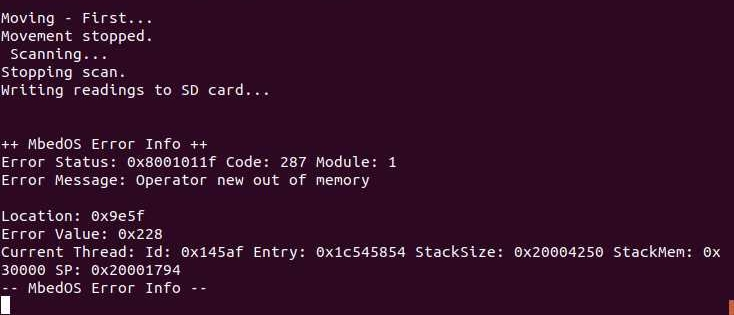
\includegraphics[width=.8\linewidth]{SYNTHESIS/memoryerror.jpg}
			\label{fig:memoryerror}
		\end{figure}
		
		This error began cropping up at the point where the program writes the buffer to a physical file. Despite it not being during the time when the readings buffer was actually filled out, the immediate reaction to the issue was simply to scale down the buffer. It made sense that perhaps too much space was being taken up by such a large variable, so it was halved to contain just 8000 angle distance pairs. The error was still encountered when compiling however, so just to see what would happen the array was decreased down to a significantly smaller size of just 1000. This issue still happened though, despite attempts to recompile and reflash the microcontroller as well as resetting the board with the reset button.
		
		\section{Scanning Inconsistency}
		One problem that repeatedly impeded development was the inconsistency in the LIDAR's scanning behaviour. Once development began to focus on writing real observational data into a buffer rather than filling it with dummy data just to prove the process, a number of issues began to crop up.
		
		The first was that occasionally entire batches of scan data would be zeroes. Every single angle and distance measurement would be a 0.0000000 float, with no changes to the buffer size making a difference. Pin connections were double checked and sometimes simply removed and plugged in again but then the scan straight after would result in the same thing happening. The troubleshooting section of the RPLIDAR A1M8 documentation was consulted. One suggestion was that the LIDAR core worked better once it had warmed up, and that it should be left spinning for a minute or so before it begins taking measurements. A simple task delay was introduced for 2 minutes before the main program loop began, but this issue would still come up sometimes. The quickest fix was generally to just recompile the program, and the issue would more often than not seemingly go away.
		
		
		
		
		